\subsection{Preparation}

Before any test was performed, each device had its latest \gls{isp}-provided firmware installed and was factory reset. Throughout the research, this is considered the baseline state of each device and represents a \gls{cpe} that had no intervention since the \gls{isp} had it installed on the customer’s home.

The firmware for each device was acquired by sending \gls{cwmp} Inform requests to the \gls{isp} \gls{acs} on behalf of the \gls{cpe} with the script of Appendix \ref{appendix:cwmp_dev_emu}. If the firmware was outdated, then a \gls{cwmp} Download Firmware Upgrade Image request would be received as the response, as shown in Figure \ref{figure:cwmp_download_firmware_upgrade_image}.

\begin{figure}[h]
    \centering
    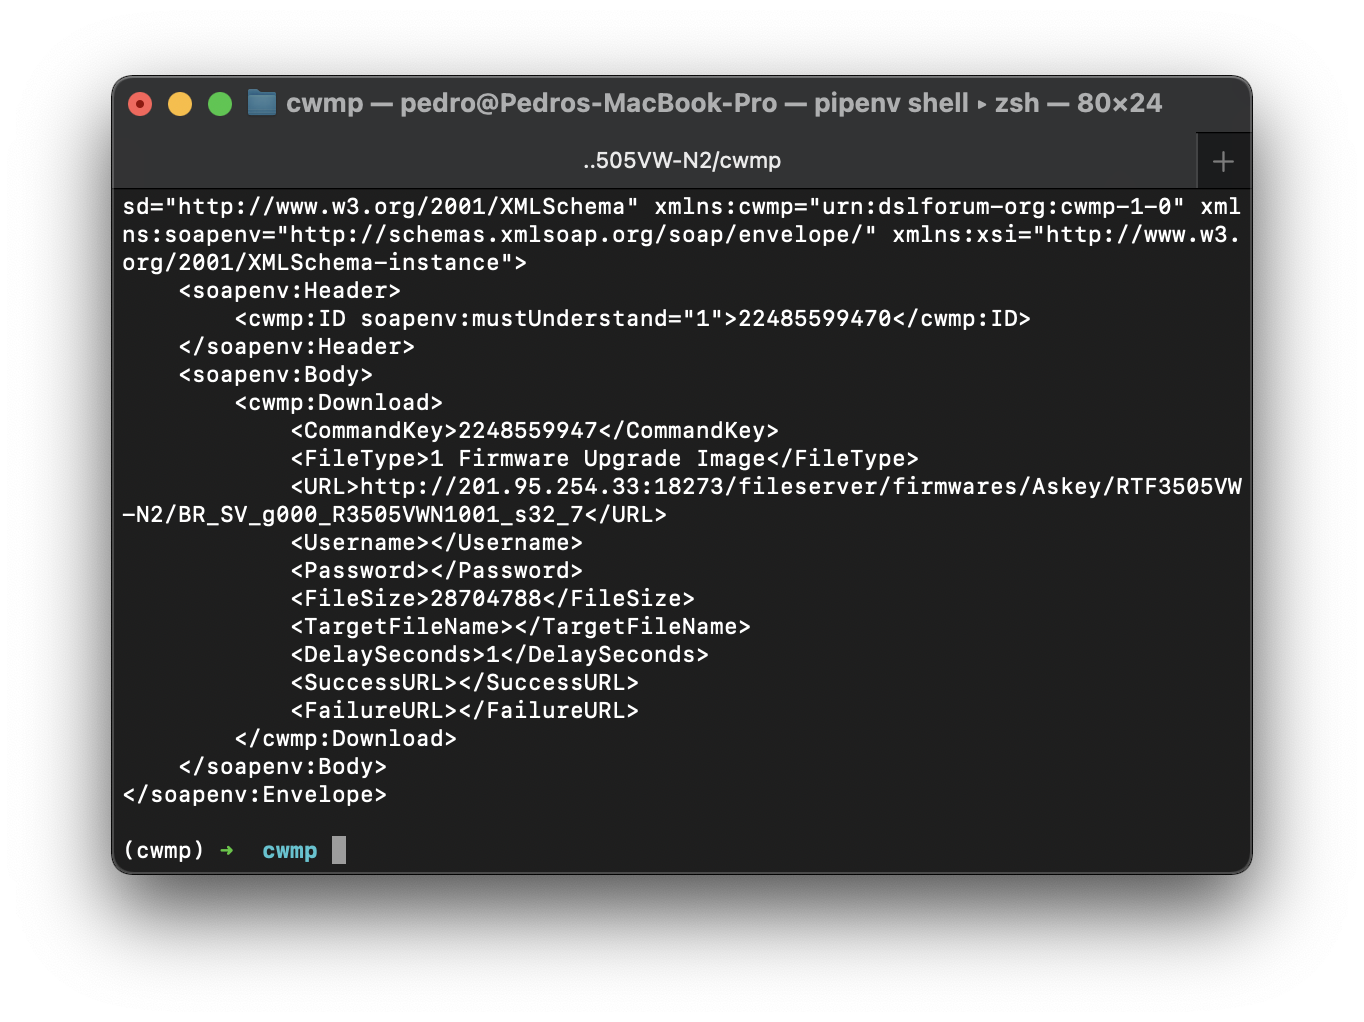
\includegraphics[width=\linewidth]{contents/cpes-and-research-data/preparation/cwmp-download-firmware-upgrade-image.png}
    \caption{\gls{cwmp} Download Firmware Upgrade Image}
    \label{figure:cwmp_download_firmware_upgrade_image}
\end{figure}

\gls{cpe}-0 and \gls{cpe}-1 never received firmware upgrade requests from \gls{acs}, no matter what version was set on the \gls{cwmp} Inform request. Looking into the firmware repository of the \gls{isp}, it was found that newer firmware was indeed available for download. But after further inspection, it was verified that both \glspl{cpe} are not able to have their firmware upgraded.

The experiments on \gls{cpe}-0 and \gls{cpe}-1 proceeded with the outdated firmware. All other devices were upgraded via the \gls{http} management interface with their respective firmware images, as shown on the Table \ref{table:cpes_firmwares}. Then, all \glspl{cpe} were factory reset by holding the reset button, located on the rear of each device, for 10 second.

\begin{table}[h]
    \makebox[\linewidth]{
        \begin{tabular}{c|c}
            \thead{\gls{cpe} Identifier} & \thead{Firmware Version} \\
            \hline
            \gls{cpe}-0 & \texttt{BR\_SO\_RTK\_V5.1.8j} \\
            \gls{cpe}-1 & \texttt{BR\_SO\_RTK\_V6.1.8t} \\
            \gls{cpe}-2 & \texttt{BR\_SA\_113WUK0b8} \\
            \gls{cpe}-3 & \texttt{BR\_SA\_g003\_114WUQ0b18} \\
            \gls{cpe}-4 & \texttt{BR\_SV\_g000\_R3505VWN1001\_s32\_7} \\
            \gls{cpe}-5 & \texttt{BR\_SG\_g11.11\_RTF\_TEF001\_V6.54\_V014} \\
            \gls{cpe}-6 & \texttt{BR\_SV\_1.00(VNZ.0)b18} \\
            \gls{cpe}-7 & \texttt{BR\_SV\_1.11(WVK.0)b18} \\
        \end{tabular}
    }
    \caption{Firmwares of the \gls{cpe}s}
    \label{table:cpes_firmwares}
\end{table}

With the devices set to their baseline, a computer was connected to one of \gls{cpe}’s \gls{lan} ports via an Ethernet cable and was able to acquire an \gls{ip} address from the \gls{dhcp} server running on the \gls{cpe}, as shown in Figure \ref{figure:wired_connection_to_the_cpe}. The gateway and \gls{dns} servers were set to the \gls{cpe}’s \gls{ip} address, \url{192.168.15.1} for all \glspl{cpe} in the research.

\begin{figure}[h]
    \centering
    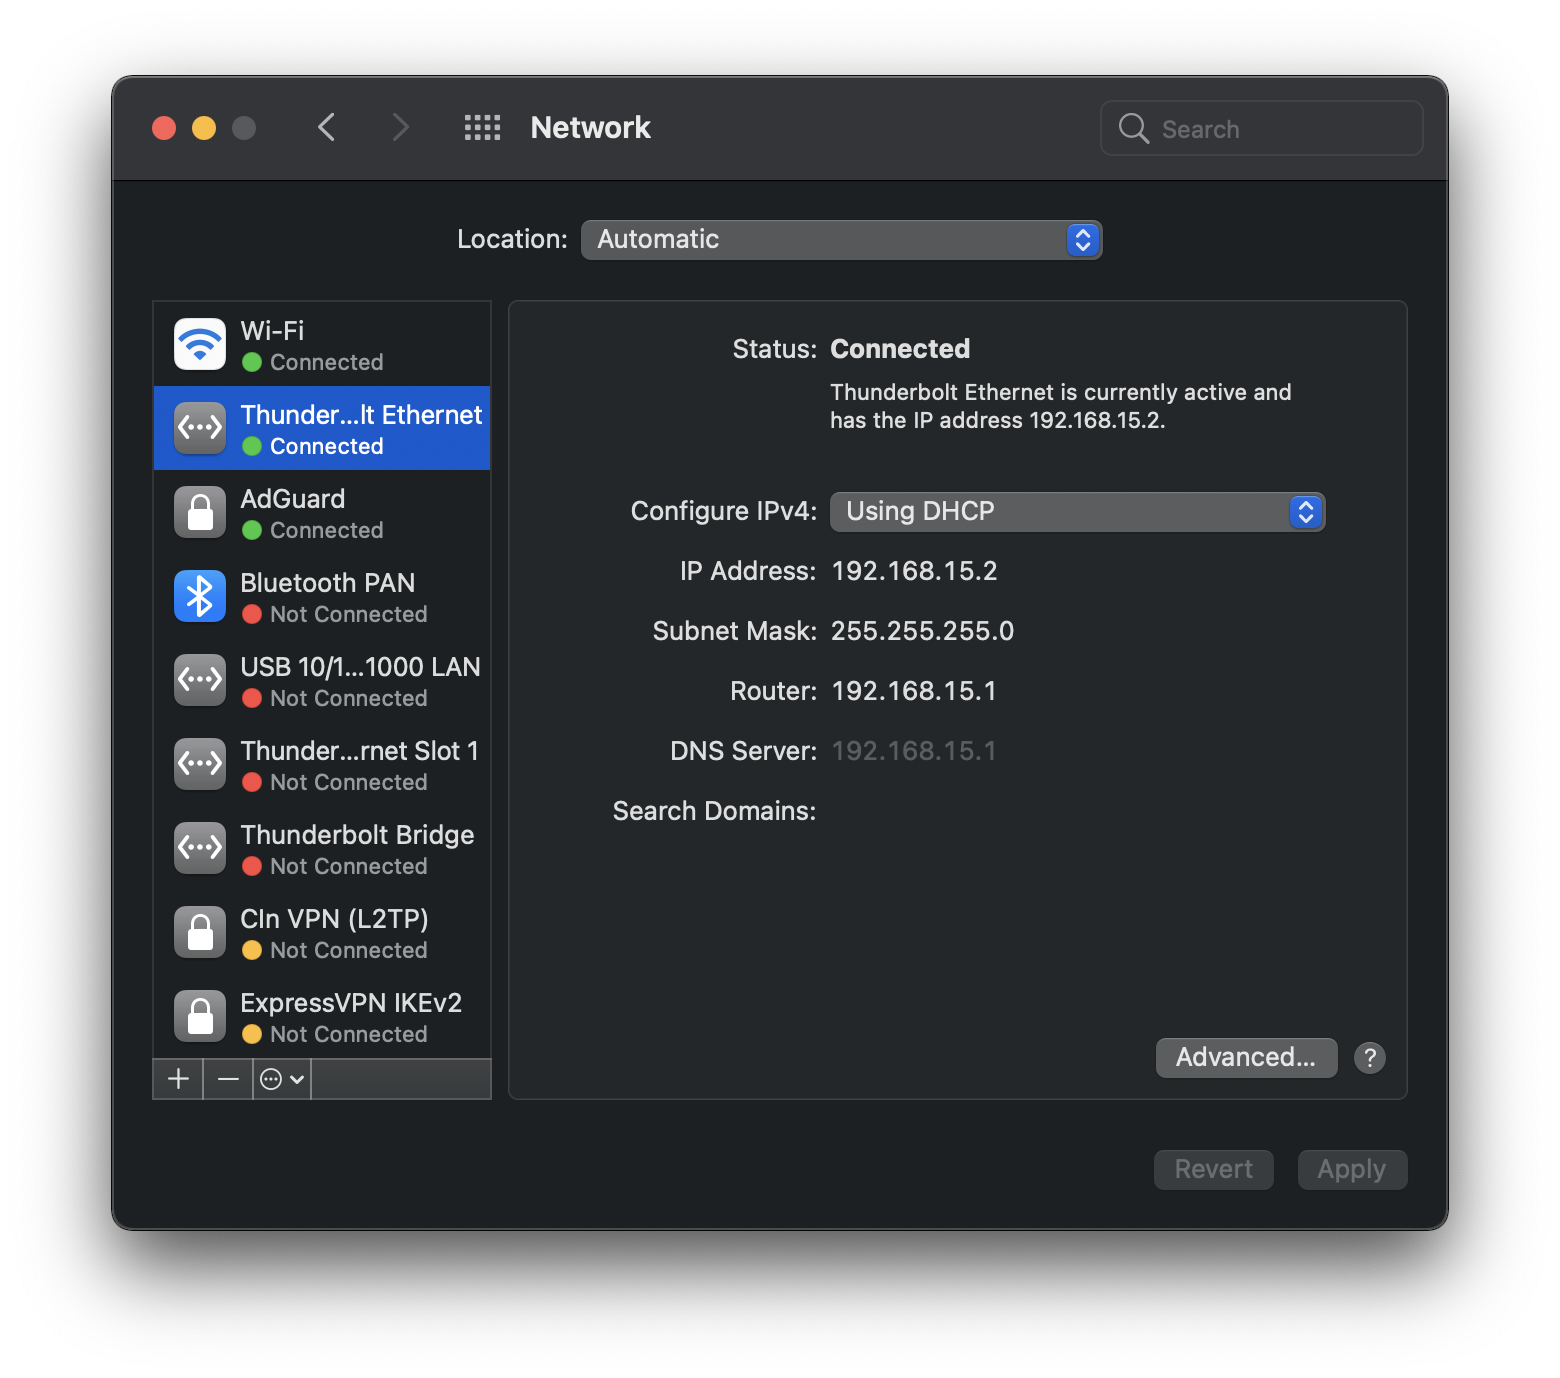
\includegraphics[width=\linewidth]{contents/cpes-and-research-data/preparation/wired-connection-to-the-cpe.png}
    \caption{Wired Connection to the \gls{cpe}}
    \label{figure:wired_connection_to_the_cpe}
\end{figure}

\FloatBarrier
